% Тут используется класс, установленный на сервере Papeeria. На случай, если
% текст понадобится редактировать где-то в другом месте, рядом лежит файл matmex-diploma-custom.cls
% который в момент своего создания был идентичен классу, установленному на сервере.
% Для того, чтобы им воспользоваться, замените matmex-diploma на matmex-diploma-custom
% Если вы работаете исключительно в Papeeria то мы настоятельно рекомендуем пользоваться
% классом matmex-diploma, поскольку он будет автоматически обновляться по мере внесения корректив
%
\documentclass{matmex-diploma-custom}

\usepackage{amsfonts}
\usepackage{amsmath}
\usepackage{hyperref}

\usepackage{listings}
\lstset{language=Java, captionpos=b, basicstyle=\footnotesize, breakatwhitespace=true, breaklines=true}
\renewcommand{\lstlistingname}{Код программы}

\begin{document}
\filltitle{ru}{
    chair              = {Кафедра Исследования Операций},
    title              = {Оконное преобразование Уолша},
    type               = {diploma},
    position           = {студента},
    group              = 523,
    author             = {Калабин Григорий Александрович},
    supervisorPosition = {к.\,ф.-м.\,н., доцент},
    supervisor         = {{\sigplace{С.М.~Машарский}{подпись}}},
    reviewerPosition   = {д.\,ф.-м.\,н., профессор},
    reviewer           = {{\sigplace{В.Н.~Малозёмов}{подпись}}},
    chairHeadPosition  = {д.\,ф.-м.\,н., профессор},
    chairHead          = {{\sigplace{И.В.~Романовский}{подпись}}},
%   university         = {Санкт-Петербургский Государственный Университет},
%   faculty            = {Математико-механический факультет},
%   city               = {Санкт-Петербург},
%   year               = {2013}
}
\filltitle{en}{
    chair              = {Chair of The Operations Research},
    title              = {Short-time Walsh transform},
    author             = {Grigory Kalabin},
    supervisorPosition = {docent},
    supervisor         = {{\sigplace{S.M.~Masharsky}{signature}}},
    reviewerPosition   = {professor},
    reviewer           = {{\sigplace{V.N.~Malozemov}{signature}}},
    chairHeadPosition  = {professor},
    chairHead          = {{\sigplace{J.V.~Romanovsky}{signature}}},
}
\maketitle
\tableofcontents
\newpage
% У введения нет номера главы
\section*{Введение}
Идея оконного преобразования давно известна~\cite{b-allen} и широко применяется в 
цифровой обработке сигналов. В частности, данный подход активно используется при
реализации эквалайзеров и построении спектрограмм, к примеру, 
специалисты по обработке аудио
используют спектрограммы для выявления частот, соответствующих каким-либо шумам
или для нахождения резонансных частот в помещении, где был записан сигнал, а с 
помощью эквалайзера можно эти частоты выровнять или вообще устранить.

Не всегда возможно работать целиком с исследуемым сигналом. Зачастую сигналы, 
которые необходимо обрабатывать, достаточно длинные. Обычно цифровое аудио имеет
частоту дискретизации 44,1~kHz, а это значит, что каждая секунда такого аудио
представляется 44 100 значениями. Таким образом, аудиофайл длительностью в пару
минут представляется 5~292~000 отсчётами. Если время обработки не так принципиально,
то можно использовать не самые оптимальные алгоритмы и подходы.

Ситуация кардинально меняется, если необходимо изменять аудио во время 
прослушивания. Это означает, что любая задержка, даже в десятую долю секунды,
становится крайне нежелательной. 
Пример подобной ситуации --- работа с эквалайзером, при которой
мы применяем различные фильтры к сигналу и хотим слышать изменения в реальном времени.
Процесс работы с эквалайзером называется \emph{эквализацией} и используется 
практически всегда при записи музыки.

Теперь представим себе ситуацию, что исследуемый сигнал начался неизвестно когда
и неизвестно когда закончится, а обрабатывать его нужно прямо сейчас. Такие ситуации
встречаются достаточно часто, например, при разговоре с удалённым 
собеседником. Помимо нашего голоса, динамики воспринимают большое количество внешних
шумов (таких как проезжающие рядом автомобили, порывы ветра или слова посторонних людей).
Ясно, что задержки при обработке сигнала в этой ситуации также нежелательны, поэтому
требования, предъявляемые к используемым подходам и алгоритмам, весьма высоки.

В этой работе рассматривается идея использования быстрого преобразования 
Уолша при оконной обработке сигнала. Такой подход позволяет не покидать вещественное
пространство при обработке вещественных сигналов, что в некоторой степени упрощает
восприятие информации, связанной со спектром исследуемого сигнала.
Также в ходе написания данной работы, оказалось, что высокие частоты спектра Уолша 
могут быть вырезаны без добавления значительного количество помех, что делает
достаточно перспективным направление сжатия сигналов на основе спектра Уолша.

Для демонстрации рассматриваемой идеи на практике были написаны два 
приложения. Одно из этих приложений --- эквалайзер, использующий
оконное преобразование Уолша для фильтрации сигнала. Другое приложение демонстрирует
возможность сжатия аудио на основе подхода, рассматриваемого в данной работе. 
Обзор этих приложений представлен в разделе~\ref{sec:demo}.

Формальные определения объектов, используемых в работе, описаны в разделе~
\ref{sec:preliminary}.


\section{Предварительные сведения}
\label{sec:preliminary}
В этом разделе представлено математическое описание объектов, используемых в работе.
Формальные определения и обозначения, связанные с сигналами,
заимствованы из книги \cite{dha}.

Носитель функции $f: \, X \rightarrow Y$ --- 
это замыкание подмножества $X$, на котором функция $f$ не обращается в ноль:
$$
 \mathrm{supp}\,f=\overline{\left\{x\mid f(x)\ne 0\right\}}.
$$

Любое число $j \in 0:2^\nu - 1$ можно представить единственным образом в виде
$$
 j = j_{\nu-1} 2^{\nu-1} + j_{\nu-2} 2^{\nu-2} + \ldots + j_1 2 + j_0,
$$
где все коэффициенты $j_k$ равны нулю или единице. Более компактная запись данного
равенства --- $j=(j_{\nu-1}, j_{\nu-2}, \ldots, j_0)_2$.

Введём обозначение  
$$
  \mathrm{rev}_\nu(j) = (j_0, j_1, \ldots, j_{\nu-1})_2.
$$

Зафиксируем натуральное число $N$. \emph{Сигналом} длины $N$ будем называть комплекснозначную 
функцию целочисленного аргумента $x = x(j), \, j \in \mathbb{N}$ с носителем $0:N-1$. 
Множество сигналов обозначим через 
$\mathbb{C}_N$. В $\mathbb{C}_N$ естественным образом вводятся две операции: 
операция сложения двух сигналов и операция умножения сигнала на комплексное число:
$$
y = x_1+x_2 \: \Leftrightarrow \: y(j) = x_1(j) + x_2(j), \: j \in \mathbb{Z};
$$
$$
y = cx \: \Leftrightarrow \: y(j) = cx(j), \: j \in \mathbb{Z}.
$$
В результате $\mathbb{C}_N$ становится линейным комплексным пространством. Нулевым
элементом в $\mathbb{C}_N$ является сигнал $\mathbb{O}$, такой, что
$\mathbb{O}(j) = 0$ при всех $j \in \mathbb{Z}$.

\emph{Потоком данных} будем называть комплекснозначную 
функцию целочисленного аргумента $x = x(j), \, j \in \mathbb{N}$.




\subsection{Дискретные функции Уолша}
Рассмотрим $N = 2^s, \; N_\nu = N/2^\nu, \; \Delta_\nu = 2^{\nu - 1}$.
Пусть 
$k,j \in 0 : \Delta_{\nu+1}-1, \; k=(k_{\nu-1},k_{\nu-2},\ldots,k_0)_2 \, , \: j=(j_{\nu-1},j_{\nu-2},\ldots,j_0)_2$. 
Положим 
$$
\{k,j\}_\nu = \sum_{\alpha=0}^{\nu-1} k_\alpha j_\alpha \; , \quad k,j \in 0: \Delta_{\nu+1} - 1.
$$
Функции 
$$
v_k(j) = (-1)^{{\{k,j\}}_s} \;, \qquad k,j \in 0:N-1
$$ 
называются \emph{дискретными функциями Уолша}. Отметим, что функции Уолша 
принимают только два значения: $+1$ и $-1$.





\subsection{Базисы Уолша-Адамара и Уолша-Пэли}
Поскольку дискретные функции Уолша образуют базис в пространстве сигналов 
$\mathbb{C}_N$ 
(математическое обоснование этого факта можно найти в книге~\cite{dha}), то 
сигнал $x$ можно представить как
$$
x = \sum_{k=0}^{N-1} X(k) v_k.
$$
Базис $v_0, v_1, \ldots, v_{N-1}$ называется \emph{базисом Уолша-Адамара}.

Известно, что частота функции $v_k$ равна $\mathrm{rev}_s(k)$. Обозначим
$\hat{v}_k = v_{\mathrm{rev}_s(k)}$. Поскольку функция $\mathrm{rev}$ является 
перестановкой множества $0:N-1$, то функции $\hat{v}_k$ тоже образуют
ортогональный базис
в пространстве $\mathbb{C}_N$. Этот базис называется \emph{базисом Уолша-Пэли}.
Разложение сигнала $x$ по базису Уолша-Пэли выглядит следующим образом:
$$
  x = \sum_{k=0}^{N-1} X(\mathrm{rev}_s(k)) \hat{v}_k.
$$

\begin{figure}
    \centering
    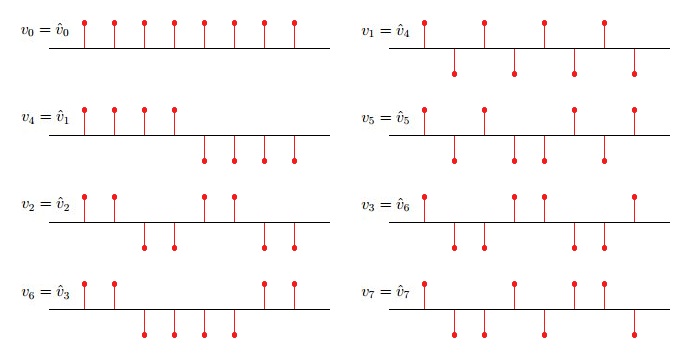
\includegraphics[width=\textwidth]{../images/walsh.png}
    \caption{Дискретные функции Уолша при $N=2^3$}
    \label{pic:функции_Уолша}
\end{figure}
При $N=2^3$ дискретные функции Уолша выглядят, как показано на рис.~\ref{pic:функции_Уолша}.





\subsection{Оконная функция}
\emph{Оконной функцией} называется весовая функция, которая равна нулю вне заданного
интервала. Например, \emph{прямоугольное окно}:
$$
w_{rect}(k) = 
\left\{ \begin{array}{ll}
  1 & \textrm{если} \; L \leq k \leq R  \\
  0 & \textrm{иначе}
\end{array} \right.
$$
где $[L;R]$ --- заданный интервал.

Ещё один пример оконной функции --- \emph{окно Хемминга}, которое задаётся формулой
$$
    w(k) = 0.5\; \left(1 - \cos \left ( \frac{2 \pi k}{N-1} \right) \right) 
$$
В этом примере носитель функции Хемминга --- $[0;N-1]$.





\section{Быстрое преобразование Уолша}
Как уже было сказано, мы хотим минимизировать задержки при обработке 
исходного сигнала.
Вычисление спектра Уолша-Пэли по определению, очевидно, имеет вычислительную 
сложность $O(N^2)$. В данной работе мы будем применять быстрый алгоритм
разложения, использующий $N \log_2 N$ сложений.

Возьмём сигнал $x \in \mathbb{C}_N$. Рекуррентные соотношения для 
последовательного вычисления коэффициентов разложения по базису Уолша
выглядят следующим образом:
\begin{gather}
\begin{split}
\label{fwt}
x_0 (k) &= x(k), \; k \in 0:N-1; \\
x_\nu (l + p \Delta_{\nu + 1}) &= 
\frac{1}{2} [ x_{\nu - 1} (l + 2 p \Delta_\nu) + x_{\nu - 1} (l + (2 p + 1) \Delta_\nu) ], \\
x_\nu (l + \Delta_\nu + p \Delta_{\nu + 1}) &= 
\frac{1}{2} [ x_{\nu - 1} (l + 2 p \Delta_\nu) - x_{\nu - 1} (l + (2 p +1) \Delta_\nu) ], 
\end{split}
\\
p \in 0:N_\nu - 1, \; l \in 0:\Delta_\nu - 1, \; \nu = 1, \ldots, s. \nonumber
\end{gather}
При $\nu = s$ получаем разложение сигнала $x$ по базису Уолша:
\begin{equation}
\label{fwtWalsh}
  x 
  = \sum_{k=0}^{N-1} x_s(k) v_k 
  = \sum_{k=0}^{N-1} x_s(\mathrm{rev}_s(k)) \hat{v}_k.
\end{equation}


Схема~(\ref{fwt}) называется \emph{быстрым преобразованием Уолша, связанным с 
прореживанием по времени}. Эта схема использует только 
сложения в количестве $N\log_2 N$ операций.

Соотношения~(\ref{fwt}) допускают обращение
\begin{gather}
\begin{split}
\label{revfwt}
x_{\nu - 1} (l + 2 p \Delta_\nu) &=
x_\nu (l + p \Delta_{\nu + 1}) + x_\nu (l + \Delta_\nu + p \Delta_{\nu + 1}), \\
x_{\nu - 1} (l + (2 p + 1) \Delta_\nu) &=
x_\nu (l + p \Delta_{\nu + 1}) - x_\nu (l + \Delta_\nu + p \Delta_{\nu + 1}),
\end{split}
\\
p \in 0:N_\nu - 1, \; l \in 0:\Delta_\nu - 1, \; \nu = s, s-1, \ldots, 1. \nonumber
\end{gather}

При этом $x(k) = x_0(k), \; k \in 0: N-1$.

Из формулы~(\ref{fwtWalsh}) видно, что быстрый алгоритм возможно использовать
для разложения сигнала по базису Уолша-Пэли.



\section{Оконное преобразование Уолша}
Далее будет рассмотрено оконное преобразование Уолша. Сначала рассмотрим общую
идею оконного преобразования, а затем дадим формальное определение.




\subsection{Общая идея оконного преобразования}
Допустим, имеется исходный поток данных, который необходимо обработать.
Общая идея оконного преобразования выглядит следующим образом:

\begin{enumerate}
  \item Зафиксируем $N, d \in \mathbb{N}$
  \item Возьмём оконную функцию $w_0$ с носителем $0:N-1$
  \item Определим сигнал $x$, как очередные $N$ отсчётов
    исходного потока данных. Умножим $x$ на $w_0$ покомпонентно. 
    Рассмотрим результат умножения
    на носителе $w_0$ ---  сигнал $x' \in \mathbb{C}_N$
  \item Произведём обработку $x'$ и получим $x'' \in \mathbb{C}_N$
  \item Запишем $x''$ в некоторый буфер
  \item Преобразуем $w_0$ в $w_1$ так, что $\mathrm{supp}\,(w_1) = d:N+d-1$. 
    Повторим шаги 3--4 для $w_1$. Результат запишем в буфер, учитывая смещение $d$
  \item Будем сдвигать носитель очередной оконной функции и 
    повторять шаги 3--6, пока не обработаем весь исходный сигнал. В результате 
    буфер будет содержать результат обработки
\end{enumerate}

Очевидно, что наличие всего потока данных в момент начала обработки
не требуется, поскольку на каждой итерации обработки очередной части потока нас интересуют
только значения потока данных на носителе окна $w$. Таким образом, данный подход позволяет
обрабатывать в реальном времени сигналы, которые неизвестно когда закончатся (например,
человеческую речь).

Также отметим, что допустимо наложение носителей оконных функций. В этом случае
 необходимо <<склеивание>> наложившихся частей. 
 Мы не будем останавливаться подробно на этом вопросе, поскольку 
в этой работе мы будем <<сдвигать>> окно на всю его длину, поэтому вопрос <<склеивания>> 
наложившихся частей для данной работы не актуален.


\subsection{Обработка сигнала}
Для того чтобы использовать спектр Уолша при обработке очередной части потока данных,
необходимо использовать длину окна $N = 2^s, \, s \in \mathbb{N}$. Если последняя
часть потока содержит меньше отсчётов, чем $N$, то можно дополнить её нулями.

Когда длина каждого обрабатываемого <<куска>> $x'$ сигнала представляется в виде
$2^s$, можно использовать дискретное преобразование Уолша для его обработки.
Будем раскладывать $x'$ по базису Уолша-Пэли и получать упорядоченный по частоте
спектр Уолша. К этому спектру мы можем применять различные фильтры для модификации
исходного сигнала. Поскольку преобразование Уолша обратимо, то 
после фильтрации вернёмся к изначальному представлению
сигнала время--амплитуда.

Если исходный сигнал является вещественным (например, аудиофайл), 
то спектр Уолша этого сигнала также будет вещественным. Это позволяет хранить 
в два раза меньше
информации для спектра
по сравнению со спектром Фурье
и упрощает представление графической информации, связанной 
с ним. Примером такой графической информации может являться спектрограмма ---
изображение, показывающее зависимость спектральной плотности мощности сигнала 
от времени. Спектрограммы применяются для идентификации речи, анализа звуков 
животных, в различных областях музыки, радио- и гидролокации, при обработке речи, 
сейсмологии и в других областях.




\subsection{Формальное определение}
Теперь дадим формальное определение оконному преобразованию Уолша. 
По соображениям, приведённым выше, мы будем использовать базис Уолша-Пэли,
однако данное определение может быть легко сформулировано и для базиса 
Уолша-Адамара.

Пусть у нас есть
некоторый поток данных $x$. И прямоугольная оконная функция $w$ с носителем
$0:N-1$.
Оконным преобразованием Уолша потока данных $x$ называется матрица $X$, задаваемая 
следующим равенством:

\[ 
\mathbf{STWT}\{x\}(d,k)\equiv X(d,k) 
= \frac{1}{N} \sum_{j=0}^{N-1} x[j+d]w[j]\hat{v}_k(j),
\quad k \in 0:N-1, \; d \in (-\infty; +\infty).
\]

Индекс $d$ матрицы соответствует точке во времени, а индекс $k$ --- частоте.
Таким образом, данная матрица позволяет по времени и частоте узнать 
магнитуду исходного сигнала.


\subsection{Восстановление исходного сигнала}
Поскольку преобразование Уолша обратимо, то мы
можем перейти от представления частота--магнитуда к представлению
время--амплитуда.

Для каждого оконного спектра $X(d, k)$ вычислим обратное преобразование
Уолша и получим часть исходного потока данных:
\[
x(d,j) = \sum_{k=0}^{N-1} X(d,k) \hat{v}_k(j),
\quad j \in 0:N-1, \; d \in (-\infty; +\infty).
\]

Поскольку в данной работе рассматривается оконное преобразование
с прямоугольным окном, то
можно перейти от матрицы $x(d,j)$ к исходному потоку данных $x(t)$ следующим образом:
\[
 x(t) = \frac{1}{N} \sum_{j=0}^{N-1} x(t-j,j), \quad t \in (-\infty; +\infty).
\]


\section{Результаты}
В рамках данной работы было реализовано оконное преобразование Уолша на языке java
и были проведены различные эксперименты. В качестве исходных данных брались
аудио файлы с записью гитары, пианино, скрипки и человеческой речи. Некоторая информация об
исходных данных указана в таблице~\ref{tab:audio-samples}.

\begin{table}
  \centering
    \begin{tabular}{ | p{2.4cm} | l | p{2cm} | p{2cm} | p{2cm} | p{4.5cm} |}
    \hline
    Название файла & Инструмент & Длитель-ность & Размер, byte & Размер, samples & Примечание \\ \hline
    vivaldi.wav & Скрипка & 15~сек & 2 921 548 & 1 460 752 & Антонио Вивальди, <<Весна>>, часть 1 Аллегро \\ \hline
    chopin.wav & Фортепиано & 13~сек & 1 178 548 & 589 203 & Фридерик Шопен, <<ноктюрн №2>> \\ \hline
    metallica.wav & Гитара & 24~сек & 2 190 902 & 1 095 429 & Группа <<Metallica>>, <<Nothing else matters>> \\ \hline
    voice.wav & Речь & 3~сек & 702 644 & 351 300 & Женская речь \\ \hline
    \end{tabular}
    \caption{Описание тестовых исходных данных}
    \label{tab:audio-samples}
\end{table}

Было установлено, что при помощь оконного преобразования Уолша возможна
достаточно эффективная обработка сигналов.

\subsection{Вырезание частот}
В рамках данной работы был проведён эксперимент в котором из спектра вырезались верхние частоты, то есть
к исходному сигналу применялся простейший низкочастотный фильтр.
При проведении эксперимента использовалось прямоугольное окно без наложений с длиной
равной 1024 отсчётам.
В результате было получено,
что при вырезании $15/16$ верхних частот, то есть обнулении компонент спектра
Уолша-Пэли с индексами от 65 до 1023, результат фильтрации вполне узнаваем.
Можно сделать вывод, что верхние частоты при разложении сигнала по
базису Уолша воспринимаются человеком значительно меньше, чем низкие.
Этот факт можно использовать для реализации сжатия на основе 
оконного преобразования Уолша.

\subsection{Сжатие звука на основе оконного преобразования Уолша}
При написании данной работы были проведены различные эксперименты
по сжатию звука с помощью оконного преобразования Уолша. Сводные результаты
экспериментов приведены в таблице~\ref{tab:compression-ratio}. 
Для сжатия данных использовался алгоритм DEFLATE~\cite{deflate-spec}.
Компрессия применялась не к каждому отдельному окну, а ко всему
сигналу целиком. Это значительно увеличивает эффективность
алгоритма сжатия.

\begin{table}
  \centering
    \begin{tabular}{ | p{2.4cm} | l | l | l | l |}
    \hline
    Файл & Без фильтрации & 1/2 спектра & 1/4 спектра & 1/8 спектра \\ \hline
    vivaldi.wav     & 1.25  & 2.32  & 4.36  & 8.21 \\ \hline
    metallica.wav   & 1.22  & 2.28  & 4.32  & 8.15 \\ \hline
    chopin.wav      & 1.21  & 2.27  & 4.31  & 8.11 \\ \hline
    voice.wav       & 1.21  & 2.26  & 4.27  & 8.10 \\ \hline
    \end{tabular}
    \caption{Коэффициент сжатия при указанной не нулевой части спектра}
    \label{tab:compression-ratio}
\end{table}




\section{Демо приложения}
\label{sec:demo}
В ходе данной работы были реализованы два приложения на языке java
для демонстрации возможностей оконного преобразования.
Весь исходный код программ можно найти по адресу \url{http://bitbucket.org/gkalabin/diploma}.
Данные приложения могут работать с аудио-файлами в формате wav. Чтение и
запись wav файлов реализована по спецификации~\cite{wav-spec}.

Перед данными приложениями не ставилась задача воспроизводить 
потоковое аудио, 
поэтому чтение и запись сигналов происходит целиком, а не частями,
однако вся обработка аудио реализована с помощью оконного преобразования
Уолша. 




\subsection{Эквалайзер}
Первым представленым в данной работе демонстрационным приложением является эквалайзер на основе 
оконного преобразования Уолша. Скриншот данного приложения изображён 
на рисунке~\ref{pic:eq-screenshot}.
\begin{figure}
    \centering
    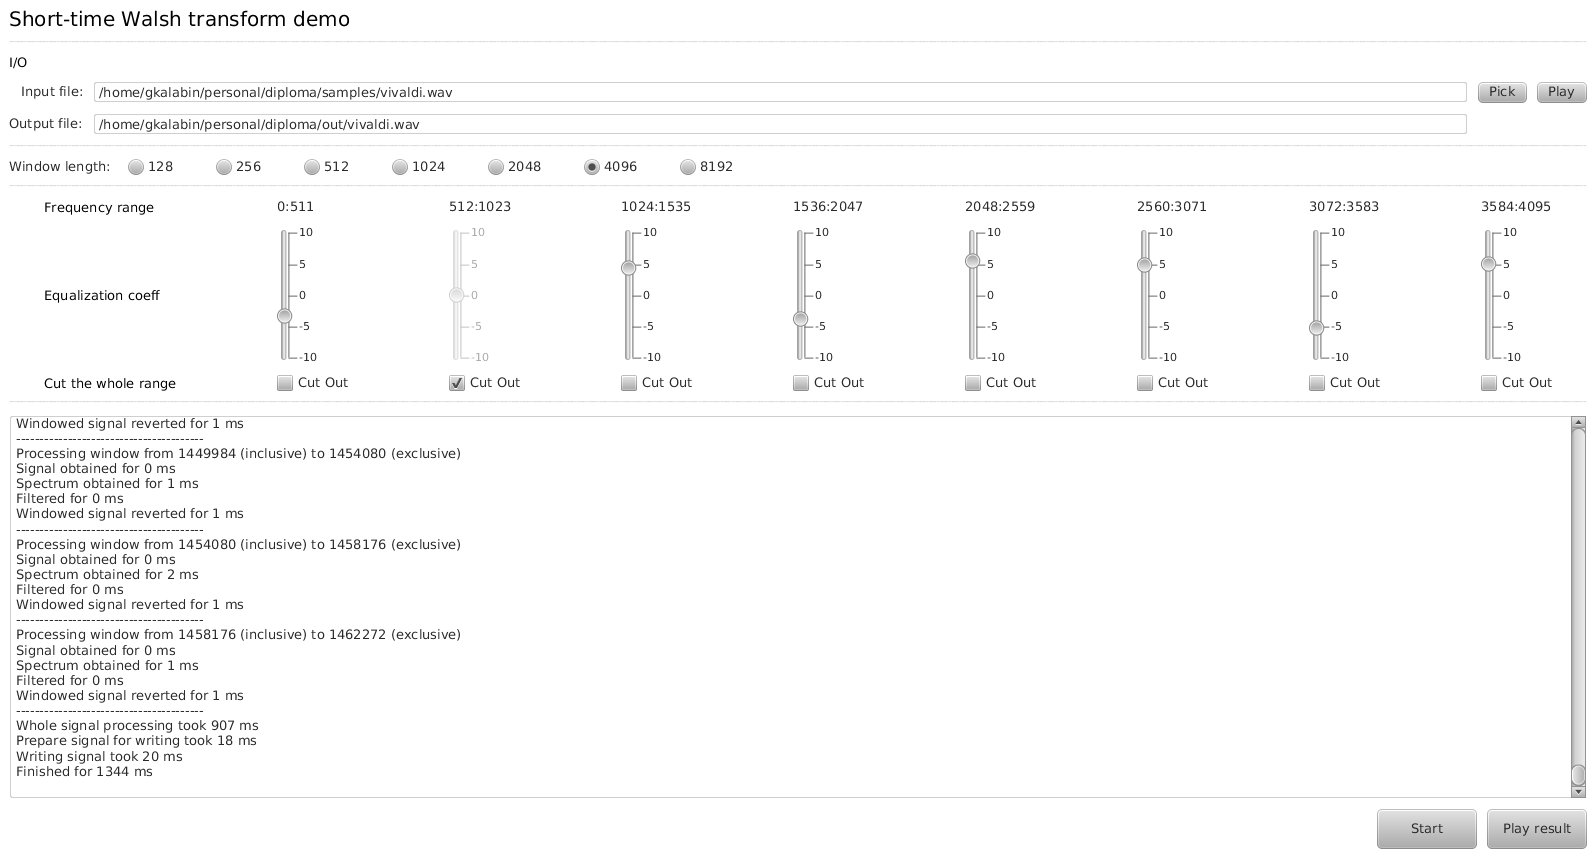
\includegraphics[width=\textwidth, keepaspectratio=true]{../images/equalizer-screen.png}
    \caption{Эквалайзер на основе оконного преобразования Уолша}
    \label{pic:eq-screenshot}
\end{figure}

В этом приложении возможно регулировать мощность 8 диапазонов частот
исходного сигнала в диапазоне от -10dB до +10dB, а также обнулять тот или иной диапазон.

Также возможен выбор длины окна, которое будет использоваться для 
обработки сигнала, в диапазоне от 128 до 8192 отсчётов.

При нажатии кнопки <<Start>> читается входной файл, производится 
его обработка, в зависимости от указанных параметров фильтрации.
Затем результат записывается в выходной файл. Также имеется возможность
прослушать входной и выходной аудио-файлы.

Детальная информация об обработке сигнала выводится в специальное
поле, которое очищается перед очередным запуском фильтрации.

\subsection{Сжатие аудио}
Другое приложение, написанное в ходе данной работы, позволяет
сжимать аудио файлы на основе оконного преобразования Уолша с использованием
алгоритма сжатия DEFLATE~\cite{deflate-spec}. Скриншот данного приложения
представлен на рисунке~\ref{pic:compressor-screenshot}.
\begin{figure}
    \centering
    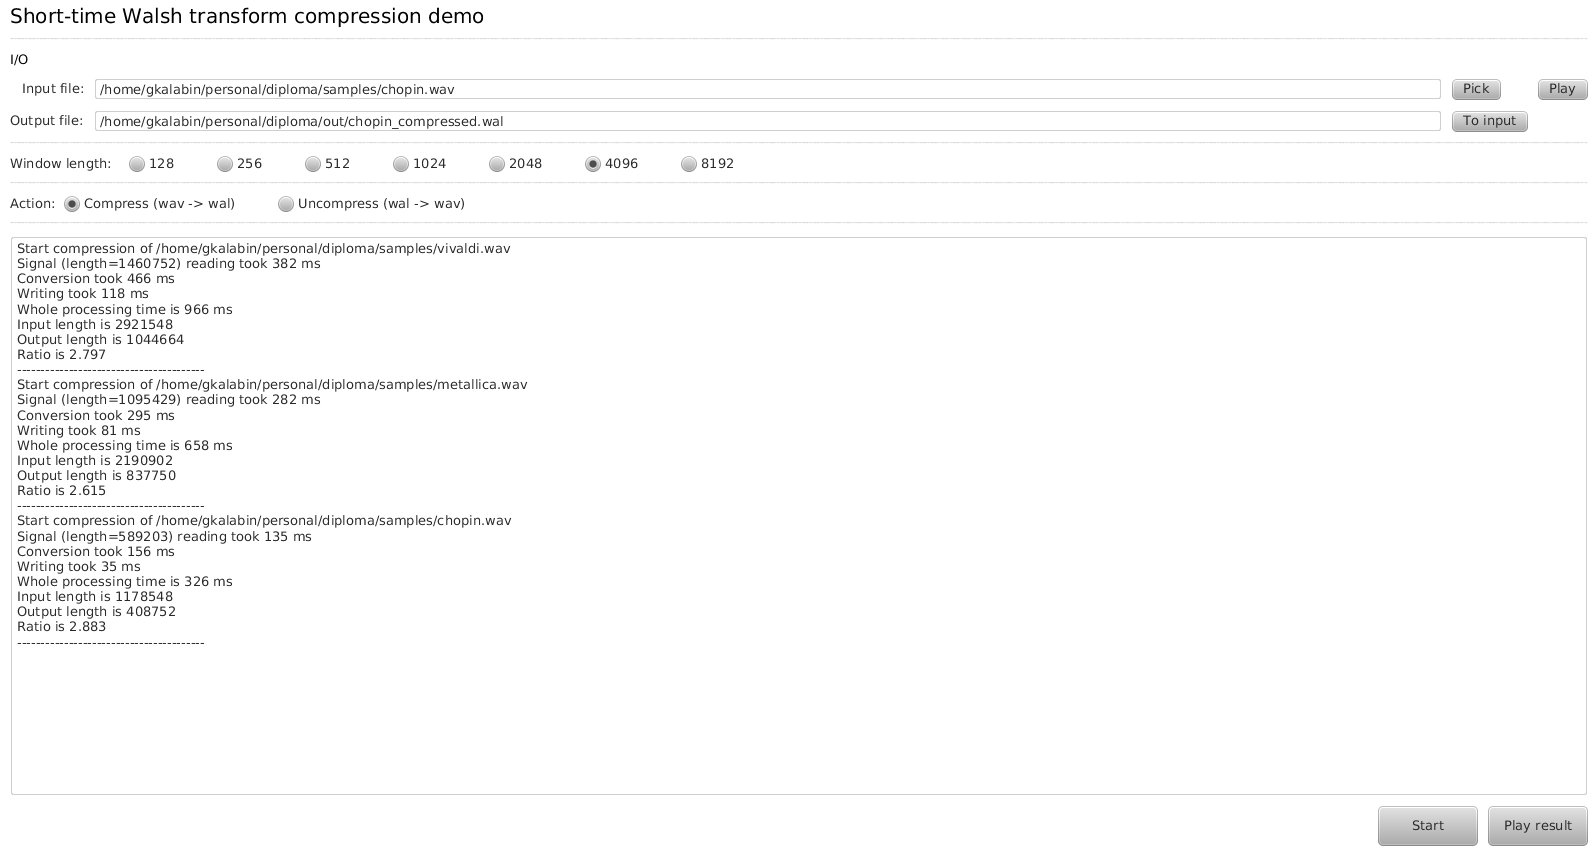
\includegraphics[width=\textwidth, keepaspectratio=true]{../images/compressor-screen.png}
    \caption{Приложение, осуществляющее сжатие на основе оконного преобразования Уолша}
    \label{pic:compressor-screenshot}
\end{figure}

Сжатое аудио данным приложением записывается в выходной файл с расширением wal.
В файле wal хранится следующая информация:
\begin{itemize}
 \item Длина окна, при которой данный файл был записан
 \item Длина исходного сигнала, записанного в файле
 \item Коэффициент нормализации для каждого окна
 \item Оконный спектр Уолша-Пэли исходного сигнала
\end{itemize}

Хранение длины исходного сигнала предотвращает удлинение сигнала, 
полученного при кодировании--раскодировании wal файла. Подобное увеличении длины
сигнала
возникает при дополнении последнего окна нулями для использования
преобразования Уолша.

При кодировании данных вычисляется коэффициент нормализации $\alpha_i$
для каждого оконного спектра. Это такое число, что компоненты нормированного 
спектра 
$\alpha_i X(\cdot,i)$ гарантированно попадают в диапазон значений, представимых
при заданном количестве байт на отсчёт. При таком подходе уменьшаются 
погрешности при переходе от вещественных компонент спектра к 
байтам, хранимым в wal файле. По нажатии кнопки <<Start>>
читается исходный файл, считается его оконный спектр Уолша и нормализуется. 
Затем этот спектр и нормализующий коэффициент 
записываются в wal файл.
  
При декодировании, читается wal файл, затем читаются оконные спектры
$X(\cdot,i)$,
их коэффициенты нормализации $\alpha_i$ и вычисляется исходный оконный спектр
$\frac{1}{\alpha_i} X(\cdot,i)$, производится обратное 
преобразование Уолша
по быстрому алгоритму~(\ref{revfwt}). Результат записывается в 
выходной wav файл.

При сжатии файла возможно выбрать длину окна, которая будет использована
при оконном преобразовании Уолша. При декодировании wal файла выбор длины окна
недопустим, поскольку длина окна хранится в wal файле.

Сообщения о результате работы программы выводятся в специальное поле.





% У заключения нет номера главы
\section*{Заключение}
В ходе данной дипломной работы была рассмотрена идея совмещения
дискретного преобразования Уолша и оконного преобразования. Рассматриваемая 
идея оказалась достаточно перспективной в различных направлениях, таких как
сжатие и обработка сигналов. 

Одно из преимуществ использования дискретного преобразования Уолша
по сравнению с дискретным преобразованием Фурье состоит в том, что
первое не выводит нас за пределы исходного пространства, то есть, если
наш исходный сигнал был вещественный, то после обработки его с помощью
дискретного преобразования Уолша, результат также будет вещественным.
Это может значительно облегчить представление информации, используемой при
работе с цифровыми сигналами. Подобное представление упростит выявление
<<нежелательных>> частоты и различных шумов в исследуемом сигнале.

Ещё одним преимуществом оконного преобразования Уолша является 
возможность обработки сигнала без ожидания окончания ввода данных.
Примеров таких ситуаций достаточно много, но, пожалуй, самый
распространённый --- различные средства связи, в которых применяется
шумо- и эхоподавление. Различная фильтрация и оптимизация сигналов
позволяет экономить на размерах каналов передачи данных, а также улучшает
восприятие звука.

В процессе написания данной работы было обнаружено, что можно достаточно 
эффективно сжимать звуковые сигналы с помощью оконного преобразования Уолша.
Для демонстрации этого факта было написано соответствующее приложение.

Для хранения сжатых аудиофайлов был написан собственный аудиокодек,
который может записывать оконный спектр Уолша в файл, а также
читать ранее записанный спектр из файла. Такие файлы записываются
с расширением \emph{wal} --- сокращённое от Walsh (Уолш).

Все цели поставленные перед написанием данной работы были достигнуты,
перспективность рассматриваемого подхода продемонстрирована, поэтому
можно считать, что исследование оконного преобразования Уолша завершено 
в рамках данной работы.



\bibliographystyle{ugost2008}
\nocite{*}
\bibliography{diploma.bib}

\begin{appendices}
\section{Исходный код программы}
    \begin{lstlisting}[caption={Упорядочивание спектра по частоте}]
private static double[] _order(double[] value, int n, int s) {
  double[] result = new double[n];
  for (int i = 0; i < n; i++) {
    result[Walsh.rev(s, i)] = value[i];
  }
  return result;
}
\end{lstlisting}

\begin{lstlisting}[caption={Быстрое преобразование Уолша}]
public static double[] fastWT(double[] signal, int n, int s) {
  double[] xPrev = new double[n];
  System.arraycopy(signal, 0, xPrev, 0, n);
  double[] xCurr = new double[n];
  int N_nu = n;
  int delta_nu = 1;
  for (int nu = 1; nu <= s; nu++) {
    N_nu /= 2;
    int next_delta_nu = delta_nu * 2;
    for (int l = 0; l < delta_nu; l++) {
      for (int p = 0; p < N_nu; p++) {
        int leftIdx = l + p * next_delta_nu;
        int idxFirstOperand = l + 2 * p * delta_nu;
        int idxSecondOperand = l + (2 * p + 1) * delta_nu;
        xCurr[leftIdx] = .5d * (xPrev[idxFirstOperand] + xPrev[idxSecondOperand]);
        xCurr[leftIdx + delta_nu] = .5d * (xPrev[idxFirstOperand] - xPrev[idxSecondOperand]);
      }
    }
    delta_nu *= 2;
    System.arraycopy(xCurr, 0, xPrev, 0, n);
  }
  return _order(xCurr, n, s);
}
\end{lstlisting}

\begin{lstlisting}[caption={Обратное быстрое преобразование Уолша}]
public static double[] fastRevWT(double[] spectrum, int n, int s) {
  double[] xPrev = new double[n];
  double[] xCurr = new double[n];
  System.arraycopy(spectrum, 0, xCurr, 0, n);
  // N_s
  int N_nu = 1;
  // delta_s
  int delta_nu = n / 2;
  for (int nu = s; nu >= 1; nu--) {
    int next_delta_nu = delta_nu * 2;
    for (int l = 0; l < delta_nu; l++) {
      for (int p = 0; p < N_nu; p++) {
        int leftIdx = l + 2 * p * delta_nu;
        int idxFirstOperand = l + p * next_delta_nu;
        int idxSecondOperand = l + p * next_delta_nu + delta_nu;
        xPrev[leftIdx] = xCurr[idxFirstOperand] + xCurr[idxSecondOperand];
        xPrev[leftIdx + delta_nu] = xCurr[idxFirstOperand] - xCurr[idxSecondOperand];
      }
    }
    N_nu *= 2;
    delta_nu /= 2;
    System.arraycopy(xPrev, 0, xCurr, 0, n);
  }
  return _order(xPrev, n, s);
}
\end{lstlisting}
    \begin{lstlisting}[caption={Вычисление дискретных функций Уолша}]
public class Walsh {
  private final int myS;

  public Walsh(int s) {
    this.myS = s;
  }

  public Function<Integer, Integer> v(final int k) {
    return new Function<Integer, Integer>() {
      @Override
      public Integer apply(Integer j) {
        return bitXor(k, j, myS) % 2 == 0 ? 1 : -1;
      }
    };
  }

  /**
   * {k,j}_v
   */
  public static int bitXor(int k, int j, int v) {
    BitSet kBits = convert(k);
    BitSet jBits = convert(j);

    int result = 0;
    for (int i = 0; i < v; i++) {
      int kBit = kBits.get(i) ? 1 : 0;
      int jBit = jBits.get(i) ? 1 : 0;
      result += kBit * jBit;
    }
    return result;
  }

  private static BitSet convert(int value) {
    BitSet bits = new BitSet();
    int index = 0;
    while (value != 0) {
      if (value % 2 != 0) {
        bits.set(index);
      }
      ++index;
      value = value >>> 1;
    }
    return bits;
  }

  private static int convert(BitSet bits) {
    int value = 0;
    for (int i = 0; i < bits.length(); ++i) {
      value += bits.get(i) ? (1L << i) : 0L;
    }
    return value;
  }

  /**
   * rev_s(k)
   */
  public static int rev(int s, int k) {
    BitSet kBits = convert(k);
    for (int i = 0, revLength = s / 2; i < revLength; i++) {
      boolean tmp = kBits.get(i);
      int idx = s - i - 1;
      kBits.set(i, kBits.get(idx));
      kBits.set(idx, tmp);
    }
    return convert(kBits);
  }
\end{lstlisting}
    \begin{lstlisting}[caption={Выбор очередной оконной функции}]
class WindowIterator implements Iterator<WindowFrame> {
  private final Window myWindow;
  private final int myFrom;
  private final int myTo;
  private int myCurrentFrameStart;

  WindowIterator(Window window, int from, int to) {
    myWindow = window;
    myFrom = from;
    myTo = to;
    myCurrentFrameStart = myFrom;
  }

  WindowIterator(Window window, int to) {
    this(window, 0, to);
  }

  @Override
  public boolean hasNext() {
    return myCurrentFrameStart < myTo;
  }

  @Override
  public WindowFrame next() {
    if (!hasNext()) {
      throw new NoSuchElementException();
    }
    WindowFrame frame = myWindow.getFrame(myCurrentFrameStart);
    myCurrentFrameStart += myWindow.getLength() * myWindow.getShift();
    return frame;
  }

  @Override
  public void remove() {
    throw new UnsupportedOperationException();
  }
}
\end{lstlisting}

\begin{lstlisting}[caption={Абстрактное окно}]
public abstract class Window {

  private final int myWindowLength;
  private final double myWindowShift;

  protected Window(int windowLength, double windowShift) {
    myWindowLength = windowLength;
    myWindowShift = windowShift;
  }

  public Iterator<WindowFrame> getFrameIterator(int from, int to) {
    return new WindowIterator(this, from, to);
  }

  public Iterator<WindowFrame> getFrameIterator(int to) {
    return new WindowIterator(this, to);
  }

  public int getLength() {
    return myWindowLength;
  }

  public double getShift() {
    return myWindowShift;
  }

  public abstract WindowFrame getFrame(int left);
}
\end{lstlisting}

\begin{lstlisting}[caption={Экземпляр оконной функции}]
public abstract class WindowFrame {
  private final int myLeft;
  private final int myRight;
  private final int myLength;

  protected WindowFrame(int left, int right) {
    myLeft = left;
    myRight = right;
    myLength = right - left;
  }

  public WalshWindowedSignal apply(Signal src) {
    double[] samples = src.get(myLeft, myRight);
    double[] windowedSamples = applyToSamples(samples);
    return new WalshWindowedSignal(windowedSamples, myLeft, myRight);
  }

  private double[] applyToSamples(double[] samples) {
    double[] windowedSamples = new double[myLength];
    for (int i = 0; i < myLength; i++) {
      windowedSamples[i] = samples[i] * value(i + myLeft);
    }
    return windowedSamples;
  }

  protected int getLeft() {
    return myLeft;
  }

  protected int getRight() {
    return myRight;
  }

  protected boolean inWindow(int t) {
    return t >= getLeft() && t < getRight();
  }

  public abstract double value(int t);
}
\end{lstlisting}

\begin{lstlisting}[caption={Прямоугольное окно}]
public class RectangularWindow extends Window {

  public RectangularWindow(int windowLength, double windowShift) {
    super(windowLength, windowShift);
  }

  @Override
  public WindowFrame getFrame(int left) {
    return new RectangularWindowFrame(left);
  }

  private class RectangularWindowFrame extends WindowFrame {

    private RectangularWindowFrame(int left) {
      super(left, left + getLength());
    }

    @Override
    public double value(int t) {
      return inWindow(t) ? 1d : 0d;
    }
  }
}
\end{lstlisting}
    \begin{lstlisting}[caption={Базовый класс для сигнала и спектра}]
public abstract class WindowedSamplesWrapper {

  private final double[] mySamples;
  private final int myLeft;
  private final int myRight;

  public WindowedSamplesWrapper(double[] samples, int left, int right) {
    Preconditions.checkArgument(samples.length == right - left);
    mySamples = samples;
    myLeft = left;
    myRight = right;
  }

  public double get(int i) {
    if (i < myLeft || i >= myRight) {
      return 0d;
    }
    return mySamples[i - myLeft];
  }

  public int getLeft() {
    return myLeft;
  }

  public int getRight() {
    return myRight;
  }

  public double[] getValue() {
    return mySamples;
  }
}
\end{lstlisting}

\begin{lstlisting}[caption={Оконный сигнал}]
public class WalshWindowedSignal extends WindowedSamplesWrapper {
  public WalshWindowedSignal(double[] samples, int left, int right) {
    super(samples, left, right);
  }

  public WalshWindowedSpectrum toSpectrum() {
    double[] samples = getValue();
    int n = samples.length;
    int s = Util.intLog2(n);
    double[] value = FWT.fastWT(samples, n, s);
    return new WalshWindowedSpectrum(value, getLeft(), getRight());
  }
}
\end{lstlisting}

\begin{lstlisting}[caption={Оконный спектр}]
public class WalshWindowedSpectrum extends WindowedSamplesWrapper {

  public WalshWindowedSpectrum(double[] samples, int left, int right) {
    super(samples, left, right);
  }

  public WalshWindowedSignal toSignal() {
    double[] samples = getValue();
    int n = samples.length;
    int s = Util.intLog2(n);
    double[] value = FWT.fastRevWT(samples, n, s);
    return new WalshWindowedSignal(value, getLeft(), getRight());
  }

  public void applyFilter(Filter filter) {
    double[] samples = getValue();
    for (int i = 0; i < samples.length; i++) {
      samples[i] = filter.apply(i, samples[i]);
    }
  }

  public void applyFilters(List<Filter> filters) {
    for (Filter filter : filters) {
      applyFilter(filter);
    }
  }
}
\end{lstlisting}

\begin{lstlisting}[caption={Исходный поток данных}]
public class Signal {
  private final double[] myValue;

  public Signal(double[] value) {
    myValue = value;
  }

  public double get(int i) {
    return i < myValue.length ? myValue[i] : 0d;
  }

  public double[] get(int left, int right) {
    Preconditions.checkArgument(left < right);
    if (right <= myValue.length) {
      return Arrays.copyOfRange(myValue, left, right);
    }
    double[] result = new double[right - left];
    Arrays.fill(result, 0d);
    System.arraycopy(myValue, left, result, 0, myValue.length - left);
    return result;
  }

  public double[] getValue() {
    return myValue;
  }

  public int getLength() {
    return myValue.length;
  }

  public Iterator<WalshWindowedSignal> getIterator(Window window) {
    return new WalshSignalIterator(this, window);
  }

  public static Signal fromWindowedSignals(List<WalshWindowedSignal> signals, int length) {
    int samplesLength = 0;
    for (WalshWindowedSignal signal : signals) {
      samplesLength = Math.max(samplesLength, signal.getRight());
    }

    double[] samples = new double[samplesLength];
    Arrays.fill(samples, 0d);
    for (WalshWindowedSignal signal : signals) {
      System.arraycopy(signal.getValue(), 0, samples, signal.getLeft(), signal.getRight() - signal.getLeft());
    }
    return new Signal(Util.trimArray(samples, length));
  }

  private static class WalshSignalIterator implements Iterator<WalshWindowedSignal> {
    private final Iterator<WindowFrame> myFrameIterator;
    private final Signal mySignal;

    private WalshSignalIterator(Signal signal, Window window) {
      mySignal = signal;
      myFrameIterator = window.getFrameIterator(mySignal.getLength());
    }

    @Override
    public boolean hasNext() {
      return myFrameIterator.hasNext();
    }

    @Override
    public WalshWindowedSignal next() {
      WindowFrame frame = myFrameIterator.next();
      return frame.apply(mySignal);
    }

    @Override
    public void remove() {
      throw new UnsupportedOperationException();
    }
  }
}
\end{lstlisting}
    \begin{lstlisting}[caption={Общий интерфейс фильтров}]
public interface Filter {
  double apply(int frequency, double magnitude);
}
\end{lstlisting}

\begin{lstlisting}[caption={Простейший среднечастотный фильтр}]
public class MediumPassFilter implements Filter {
  private final int myMinFrequency;
  private final int myMaxFrequency;
  private final double myCoefficient;

  public MediumPassFilter(int minFrequency, int maxFrequency, double coefficient) {
    myMinFrequency = minFrequency;
    myMaxFrequency = maxFrequency;
    myCoefficient = coefficient;
  }

  public MediumPassFilter(int minFrequency, int maxFrequency) {
    this(minFrequency, maxFrequency, 0);
  }

  @Override
  public double apply(int frequency, double magnitude) {
    return frequency < myMinFrequency || frequency >= myMaxFrequency ? magnitude : magnitude * myCoefficient;
  }
}
\end{lstlisting}
    \begin{lstlisting}[caption={Чтение wav файлов}]
public class AudioSampleReader {

  private AudioInputStream audioInputStream;
  private AudioFormat format;

  public AudioSampleReader(File file) throws UnsupportedAudioFileException, IOException {
    audioInputStream = AudioSystem.getAudioInputStream(file);
    format = audioInputStream.getFormat();
  }

  public double[] getInterleavedSamples() throws IOException,
      IllegalArgumentException {
    // allocate a byte buffer
    byte[] inBuffer = readBytesAndCloseStream();


    // decode bytes into samples. Supported encodings are:
    // PCM-SIGNED, PCM-UNSIGNED, A-LAW, U-LAW
    return decodeBytes(inBuffer);
  }

  protected AudioInputStream getAudioInputStream() {
    return audioInputStream;
  }

  protected byte[] readBytesAndCloseStream() throws IOException {
    byte[] result = ByteStreams.toByteArray(audioInputStream);
    audioInputStream.close();
    return result;
  }

  protected double[] decodeBytes(byte[] audioBytes) {
    int sampleSizeInBytes = format.getSampleSizeInBits() / 8;
    int[] sampleBytes = new int[sampleSizeInBytes];
    double[] audioSamples = new double[audioBytes.length / sampleSizeInBytes];
    int k = 0; // index in audioBytes
    for (int i = 0; i < audioSamples.length; i++) {
      // collect sample byte in big-endian order
      if (format.isBigEndian()) {
        // bytes start with MSB
        for (int j = 0; j < sampleSizeInBytes; j++) {
          sampleBytes[j] = audioBytes[k++];
        }
      } else {
        // bytes start with LSB
        for (int j = sampleSizeInBytes - 1; j >= 0; j--) {
          sampleBytes[j] = audioBytes[k++];
        }
      }
      // get integer value from bytes
      int ival = 0;
      for (int j = 0; j < sampleSizeInBytes; j++) {
        ival += sampleBytes[j];
        if (j < sampleSizeInBytes - 1) ival <<= 8;
      }
      // decode value
      double ratio = Math.pow(2d, format.getSampleSizeInBits() - 1d);
      double val = ((double) ival) / ratio;
      audioSamples[i] = val;
    }
    return audioSamples;
  }
}
\end{lstlisting}

\begin{lstlisting}[caption={Запись wav файлов}]
public class AudioSampleWriter {

  private File file;
  private AudioFormat format;
  private AudioFileFormat.Type targetType;

  public AudioSampleWriter(File file, AudioFormat format,
                           AudioFileFormat.Type targetType) throws IOException {
    this.format = format;
    this.targetType = targetType;
    this.file = file;
  }


  public void writeInterleavedSamples(double[] interleavedSamples) throws IOException {
    byte[] bytes = encodeSamples(interleavedSamples);

    Closer closer = Closer.create();
    try {
      ByteArrayInputStream inputStream = closer.register(new ByteArrayInputStream(bytes));
      AudioInputStream audioInputStream = closer.register(new AudioInputStream(inputStream, format, AudioSystem.NOT_SPECIFIED));
      AudioSystem.write(audioInputStream, targetType, file);
    } catch (Throwable t) {
      closer.rethrow(t);
    } finally {
      closer.close();
    }
  }

  protected byte[] encodeSamples(double[] audioData) throws IOException {
    byte[] audioBytes = new byte[audioData.length * (format.getSampleSizeInBits() / 8)];
    int in;
    if (format.getSampleSizeInBits() == 16) {
      if (format.isBigEndian()) {
        for (int i = 0; i < audioData.length; i++) {
          in = (int) (audioData[i] * 32768d);
                    /* First byte is MSB (high order) */
          audioBytes[2 * i] = (byte) (in >> 8);
                    /* Second byte is LSB (low order) */
          audioBytes[2 * i + 1] = (byte) (in & 255);
        }
      } else {
        for (int i = 0; i < audioData.length; i++) {
          in = (int) (audioData[i] * 32768d);
                    /* First byte is LSB (low order) */
          byte firstByte = (byte) (in & 255);
          audioBytes[2 * i] = firstByte;
                    /* Second byte is MSB (high order) */
          audioBytes[2 * i + 1] = (byte) ((in - firstByte) >> 8);
        }
      }
    return audioBytes;
  }
}
\end{lstlisting}

\begin{lstlisting}[caption={Чтение wal файла}]
public class WalSampleReader extends AudioSampleReader {

  private int myWindowLength;
  private int mySigLength;

  public WalSampleReader(File file) throws UnsupportedAudioFileException, IOException {
    super(file);
  }

  @Override
  protected byte[] readBytesAndCloseStream() throws IOException {
    byte[] bytes = inflate(getAudioInputStream());
    ByteBuffer sigLengthBuffer = ByteBuffer.wrap(Arrays.copyOfRange(bytes, 0, 4));
    mySigLength = sigLengthBuffer.getInt();
    ByteBuffer windowLengthBuffer = ByteBuffer.wrap(Arrays.copyOfRange(bytes, 4, 8));
    myWindowLength = windowLengthBuffer.getInt();
    return Arrays.copyOfRange(bytes, 8, bytes.length);
  }

  @Override
  protected double[] decodeBytes(byte[] audioBytes) {
    int samplesCount = (int) (audioBytes.length / (WalSampleWriter.BYTES_PER_SAMPLE + 8d / myWindowLength));
    int windowCount = samplesCount / myWindowLength;
    int bytesPerWindow = 8 + myWindowLength * WalSampleWriter.BYTES_PER_SAMPLE;
    double[] audioSamples = new double[samplesCount];

    for (int windowIdx = 0; windowIdx < windowCount; windowIdx++) {
      int byteIdx = windowIdx * bytesPerWindow;
      double ratio = ByteBuffer.wrap(Arrays.copyOfRange(audioBytes, byteIdx, byteIdx + 8)).getDouble();
      byteIdx += 8;

      for (int sampleIdx = windowIdx * myWindowLength; sampleIdx < (windowIdx + 1) * myWindowLength; sampleIdx++) {
        byte[] sampleBytes = Arrays.copyOfRange(audioBytes, byteIdx, byteIdx + 2);
        byteIdx += 2;

        short ival = ByteBuffer.wrap(sampleBytes).getShort();
        // decode value
        double val = ((double) ival) / ratio;
        audioSamples[sampleIdx] = val;
      }
    }
    return audioSamples;
  }

  private static byte[] inflate(InputStream contentStream) throws IOException {
    Closer closer = Closer.create();
    try {
      BufferedInputStream bufferedStream = closer.register(new BufferedInputStream(closer.register(contentStream)));
      ObjectInputStream ois = closer.register(new ObjectInputStream(closer.register(new InflaterInputStream(bufferedStream))));
      return (byte[]) ois.readObject();
    } catch (Throwable e) {
      throw closer.rethrow(e);
    } finally {
      closer.close();
    }
  }
}
\end{lstlisting}

\begin{lstlisting}[caption={Запись wal файла}]
public class WalSampleWriter extends AudioSampleWriter {

  private final int myWindowLength;
  private final int mySigLength;
  static final int BYTES_PER_SAMPLE = 2;

  public WalSampleWriter(File file, AudioFormat format,
                         AudioFileFormat.Type targetType, int windowLength, int sigLength) throws IOException {
    super(file, format, targetType);
    myWindowLength = windowLength;
    mySigLength = sigLength;
  }

  @Override
  protected byte[] encodeSamples(double[] audioData) throws IOException {
    // encode samples as usual
    byte[] audioBytes = encodeAudioSamples(audioData);

    // put window length
    ByteBuffer windowLengthConverter = ByteBuffer.allocate(4);
    windowLengthConverter.putInt(myWindowLength);

    // put src signal length
    ByteBuffer sigLengthConverter = ByteBuffer.allocate(4);
    sigLengthConverter.putInt(mySigLength);

    byte[] result = new byte[audioBytes.length + 8];
    System.arraycopy(sigLengthConverter.array(), 0, result, 0, 4);
    System.arraycopy(windowLengthConverter.array(), 0, result, 4, 4);
    System.arraycopy(audioBytes, 0, result, 8, audioBytes.length);

    // then deflate it
    return deflate(result);
  }

  private byte[] encodeAudioSamples(double[] audioData) throws IOException {
    int windowCount = audioData.length / myWindowLength;
    byte[] audioBytes = new byte[audioData.length * BYTES_PER_SAMPLE + windowCount * 8];

    int byteIdx = 0;
    for (int i = 0; i < windowCount; i++) {
      int winStart = i * myWindowLength;
      int winEnd = (i + 1) * myWindowLength;

      double max = -1;
      for (int j = winStart; j < winEnd; j++) {
        double sample = Math.abs(audioData[j]);
        if (max < sample) {
          max = sample;
        }
      }

      double ratio = Short.MAX_VALUE / max;
      byte[] ratioBytes = ByteBuffer.allocate(8).putDouble(ratio).array();
      System.arraycopy(ratioBytes, 0, audioBytes, byteIdx, 8);
      byteIdx += 8;

      for (int j = winStart; j < winEnd; j++) {
        short in = (short) Math.round(audioData[j] * ratio);
        byte[] bytes = ByteBuffer.allocate(2).putShort(in).array();
        System.arraycopy(bytes, 0, audioBytes, byteIdx, 2);
        byteIdx += 2;
      }
    }
    return audioBytes;
  }

  private static byte[] deflate(byte[] content) throws IOException {
    Deflater deflater = new Deflater(Deflater.BEST_SPEED);
    Closer closer = Closer.create();
    try {
      ByteArrayOutputStream buffer = closer.register(new ByteArrayOutputStream());
      DeflaterOutputStream dos = closer.register(new DeflaterOutputStream(buffer, deflater));
      ObjectOutputStream oos = closer.register(new ObjectOutputStream(dos));
      oos.writeObject(content);
      oos.flush();
      oos.close();
      return buffer.toByteArray();
    } catch (Throwable e) {
      throw closer.rethrow(e);
    } finally {
      closer.close();
    }
  }
}
\end{lstlisting}
\end{appendices}
\end{document}